\section{Logic Circuits}

We can use the logic gate introduced in section 2.5 to create \textit{logic circuits}
- circuits that compute some Boolean complex function. For example, we can produce
a logic circuit that computes the sum of two bits.

As we have noted in section 2.2 the rules of addition are:

\begin{enumerate}
    \item $0 + x = x$
    \item $1 + 1 = 0\text{ carrying }1$
\end{enumerate}

Note that the sum $S$ can be produced by the XOR gate and the carry $C$ with the AND gate. Putting those
two components together we get the following circuit. This digtal logic circuit is called \textit{half adder}.
Why is it called the \textit{half} adder? This is because this circuit is not aware of any previous carry, thus
not a \textit{complete} circuit.

As we have seen from section 2.2 carrying is very important to the calculation of the sum.

\begin{figure}[ht]
    \centering
    \begin{circuitikz}
        \draw (0, 4)node[xor port] (xor){}
        (0, 2)node[and port] (and){}
        (xor.in 1) node[left=0.5cm](a) {$a$}
        (xor.in 2) node[left=0.5cm](b) {$b$}
        
        (a.east) to[short,-*] (xor.in 1) |- (and.in 1)
        (b.east) to[short,-*] ($(b.east)!.5!(xor.in 2)$) coordinate (branch)
            -- (xor.in 2)
        (branch) |- (and.in 2);
        \draw (xor.out) node[right] {$S$};
        \draw (and.out) node[right] {$C$};
    \end{circuitikz}
    \caption{The logic circuit of the half adder}
\end{figure}

\begin{table}[ht]
    \centering
    \begin{tabular}{cc|cc}
        $a$ & $b$ & $S$ & $C$ \\
        \hline
        $0$ & $0$ & $0$ & $0$ \\
        $0$ & $1$ & $1$ & $0$ \\
        $1$ & $0$ & $1$ & $0$ \\
        $1$ & $1$ & $0$ & $1$ \\
    \end{tabular}
    \caption{The truth table of the half adder}
\end{table}

The circuit that does take into account for a previous carry bit is called the \textit{full adder}.
The previous carry is called the \textit{carry-in} bit and it's the third input for this circuit.

\begin{figure}[ht]
    \centering
    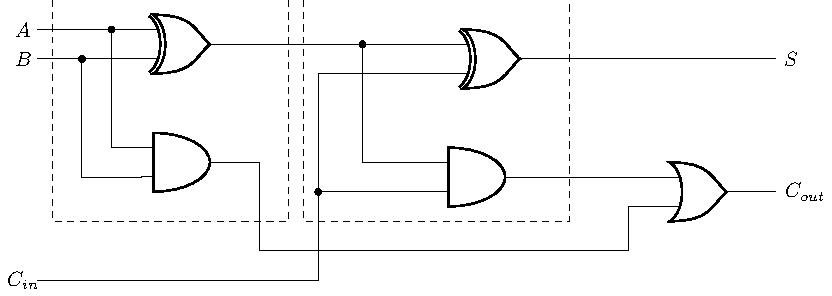
\includegraphics{images/5_Implementation/classical_fulladder_diagram.pdf}
    \caption{The logic circuit of the full adder using two half adders}
\end{figure}

\begin{table}[ht]
    \centering
    \begin{tabular}{ccc|cc}
        $a$ & $b$ & $C_{in}$ & $S$ & $C_{out}$ \\
        \hline
        $0$ & $0$ & $0$ & $0$ & $0$ \\
        $0$ & $1$ & $0$ & $1$ & $0$ \\
        $1$ & $0$ & $0$ & $1$ & $0$ \\
        $1$ & $1$ & $0$ & $0$ & $1$ \\
        $0$ & $0$ & $1$ & $1$ & $0$ \\
        $0$ & $1$ & $1$ & $0$ & $1$ \\
        $1$ & $0$ & $1$ & $0$ & $1$ \\
        $1$ & $1$ & $1$ & $1$ & $1$ \\
    \end{tabular}
    \caption{The truth table of the full adder}
\end{table}

We can see by the diagrams that the full adder circuit can be made out of
two half adder circuits. These kind of circuits, that are made from other
simple circuit, are called \textit{combinational circuits}.

By placing full adders in sequence we can make another combinational circuit
called the \textit{ripple carry adder}. This circuit can compute the sum
of $n$-bit inputs. It's called a \textit{ripple} carry adder because in order
to compute the $n$-th sum bit the circuit must first compute the $n-1$-th
sum bit thus some latency is present on the circuit. We must note at this point
that there are other better implementations of $n$-bit adders but it is out of
the scope of this work.

\begin{figure}[ht]
    \centering
    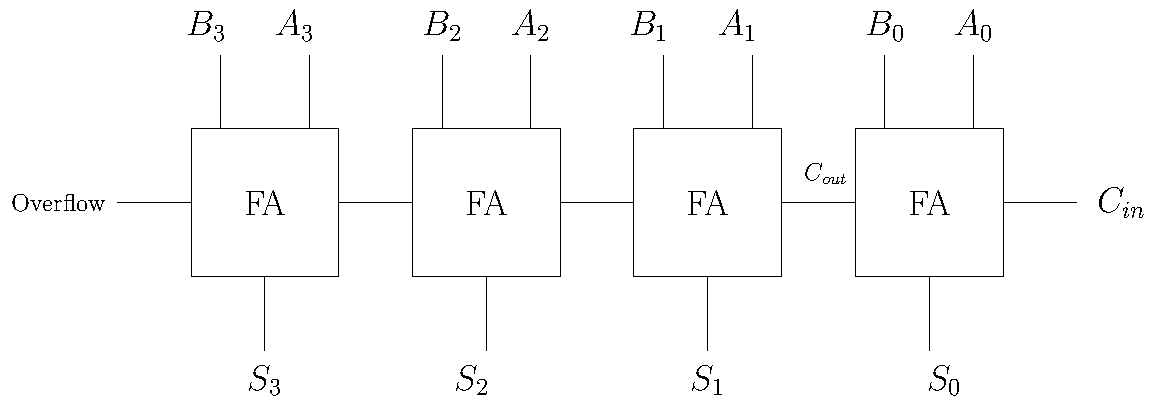
\includegraphics[width=14cm]{images/2_Classical_Computing/ripple_carry_adder.pdf}
    \caption{The logic circuit of a 4-bit ripple carry adder}
\end{figure}